% Options for packages loaded elsewhere
\PassOptionsToPackage{unicode}{hyperref}
\PassOptionsToPackage{hyphens}{url}
\PassOptionsToPackage{dvipsnames,svgnames*,x11names*}{xcolor}
%
\documentclass[
  12pt,
  ,
  a4paper]{article}
\usepackage{lmodern}
\usepackage{amssymb,amsmath}
\usepackage{ifxetex,ifluatex}
\ifnum 0\ifxetex 1\fi\ifluatex 1\fi=0 % if pdftex
  \usepackage[T1]{fontenc}
  \usepackage[utf8]{inputenc}
  \usepackage{textcomp} % provide euro and other symbols
\else % if luatex or xetex
  \usepackage{unicode-math}
  \defaultfontfeatures{Scale=MatchLowercase}
  \defaultfontfeatures[\rmfamily]{Ligatures=TeX,Scale=1}
\fi
% Use upquote if available, for straight quotes in verbatim environments
\IfFileExists{upquote.sty}{\usepackage{upquote}}{}
\IfFileExists{microtype.sty}{% use microtype if available
  \usepackage[]{microtype}
  \UseMicrotypeSet[protrusion]{basicmath} % disable protrusion for tt fonts
}{}
\makeatletter
\@ifundefined{KOMAClassName}{% if non-KOMA class
  \IfFileExists{parskip.sty}{%
    \usepackage{parskip}
  }{% else
    \setlength{\parindent}{0pt}
    \setlength{\parskip}{6pt plus 2pt minus 1pt}}
}{% if KOMA class
  \KOMAoptions{parskip=half}}
\makeatother
\usepackage{xcolor}
\IfFileExists{xurl.sty}{\usepackage{xurl}}{} % add URL line breaks if available
\IfFileExists{bookmark.sty}{\usepackage{bookmark}}{\usepackage{hyperref}}
\hypersetup{
  pdftitle={Rapport},
  pdfauthor={Alain Quartier-la-Tente},
  pdflang={english},
  colorlinks=true,
  linkcolor=Maroon,
  filecolor=Maroon,
  citecolor=Blue,
  urlcolor=blue,
  pdfcreator={LaTeX via pandoc}}
\urlstyle{same} % disable monospaced font for URLs
\usepackage[margin=1in]{geometry}
\usepackage{longtable,booktabs}
% Correct order of tables after \paragraph or \subparagraph
\usepackage{etoolbox}
\makeatletter
\patchcmd\longtable{\par}{\if@noskipsec\mbox{}\fi\par}{}{}
\makeatother
% Allow footnotes in longtable head/foot
\IfFileExists{footnotehyper.sty}{\usepackage{footnotehyper}}{\usepackage{footnote}}
\makesavenoteenv{longtable}
\usepackage{graphicx,grffile}
\makeatletter
\def\maxwidth{\ifdim\Gin@nat@width>\linewidth\linewidth\else\Gin@nat@width\fi}
\def\maxheight{\ifdim\Gin@nat@height>\textheight\textheight\else\Gin@nat@height\fi}
\makeatother
% Scale images if necessary, so that they will not overflow the page
% margins by default, and it is still possible to overwrite the defaults
% using explicit options in \includegraphics[width, height, ...]{}
\setkeys{Gin}{width=\maxwidth,height=\maxheight,keepaspectratio}
% Set default figure placement to htbp
\makeatletter
\def\fps@figure{htbp}
\makeatother
\setlength{\emergencystretch}{3em} % prevent overfull lines
\providecommand{\tightlist}{%
  \setlength{\itemsep}{0pt}\setlength{\parskip}{0pt}}
\setcounter{secnumdepth}{5}
%début contraintes ensae
\usepackage{pdfpages, setspace, mathptmx} %times roman
\onehalfspacing 
\makeatletter
\def\@maketitle{%
  \newpage\setcounter{page}{0} % pour que la page d'après soit la page 1
  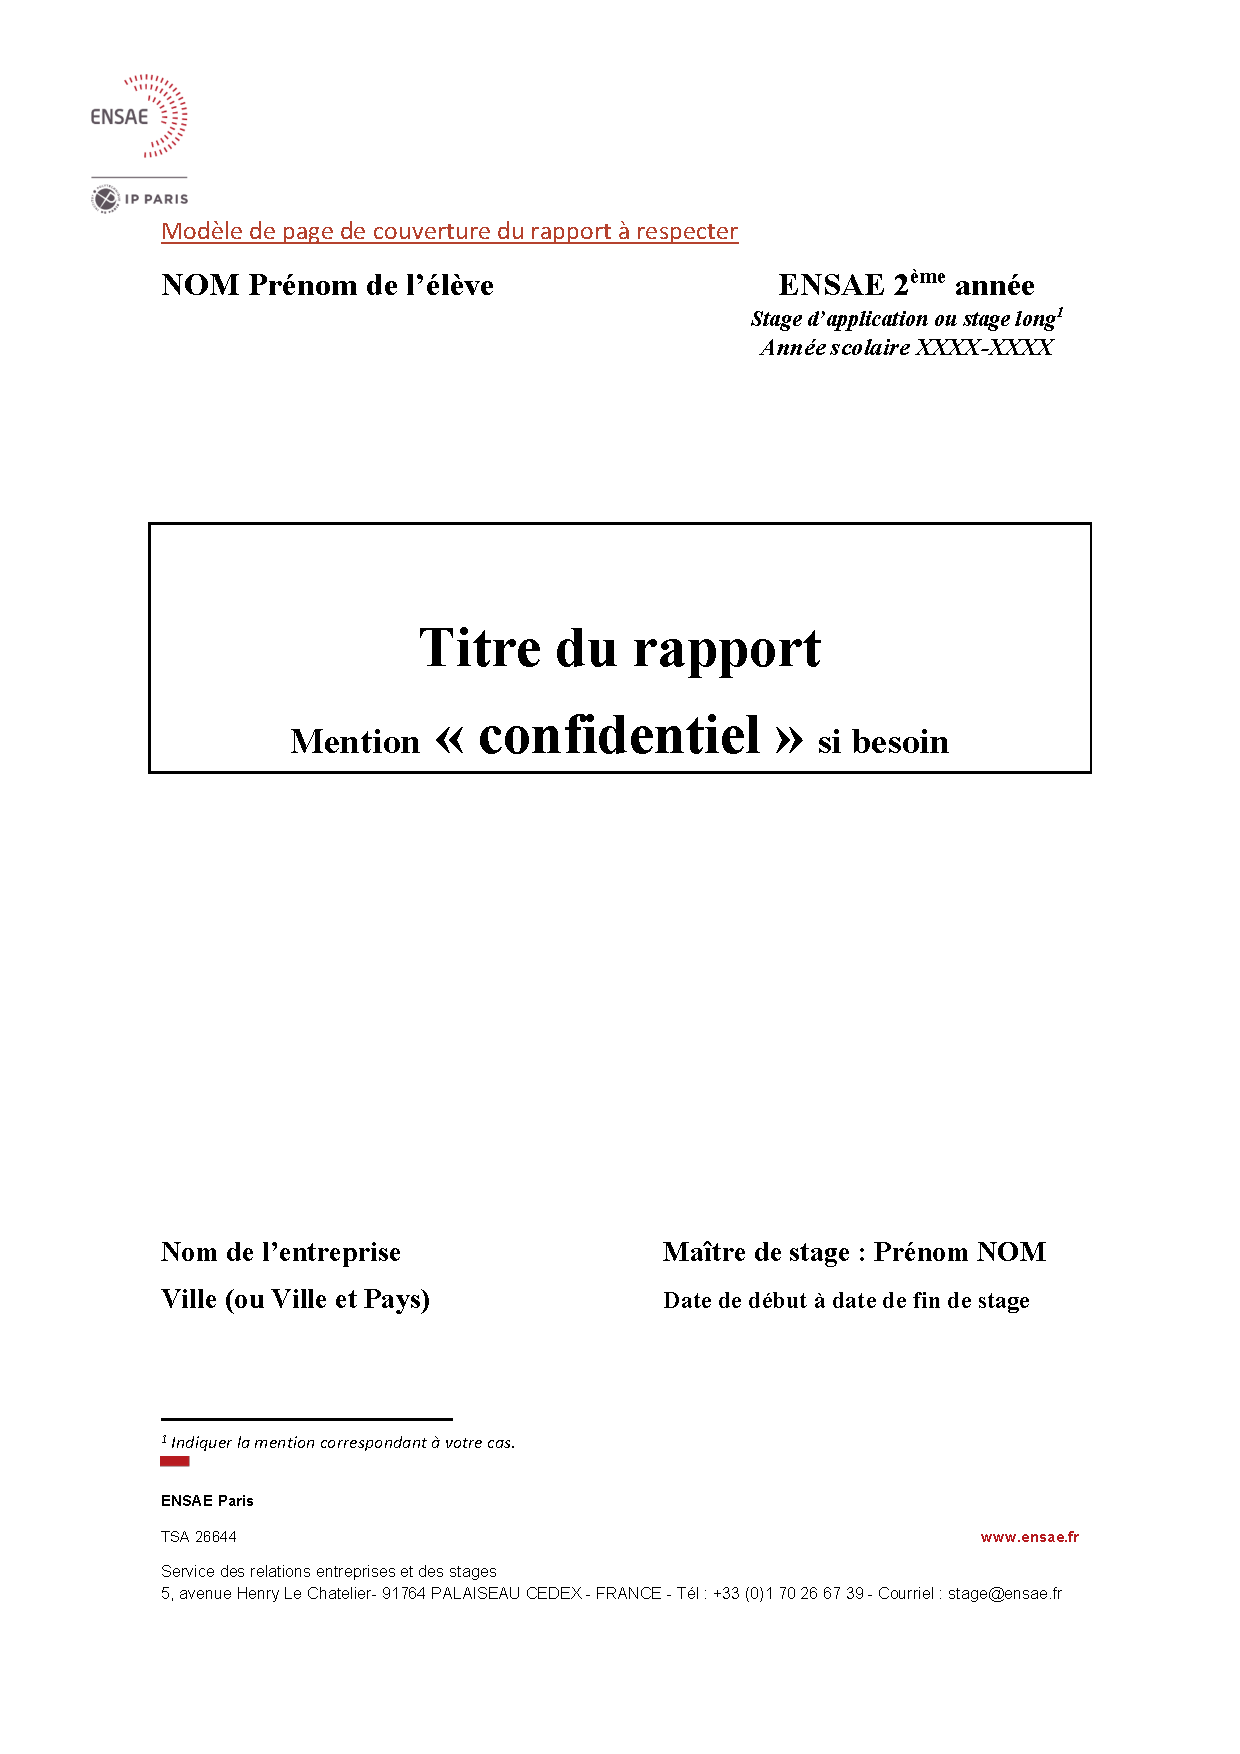
\includepdf[fitpaper=true, pages=-]{img/pdg.pdf}
}
\makeatother% cinsérer page de garde

\usepackage{stmaryrd}
\usepackage{multicol}
\usepackage{graphicx}
\usepackage{animate, dsfont, here, xspace}
%\usepackage{tikz}       
\usepackage{tikz,pgfplots}
 \pgfplotsset{compat=1.17}
%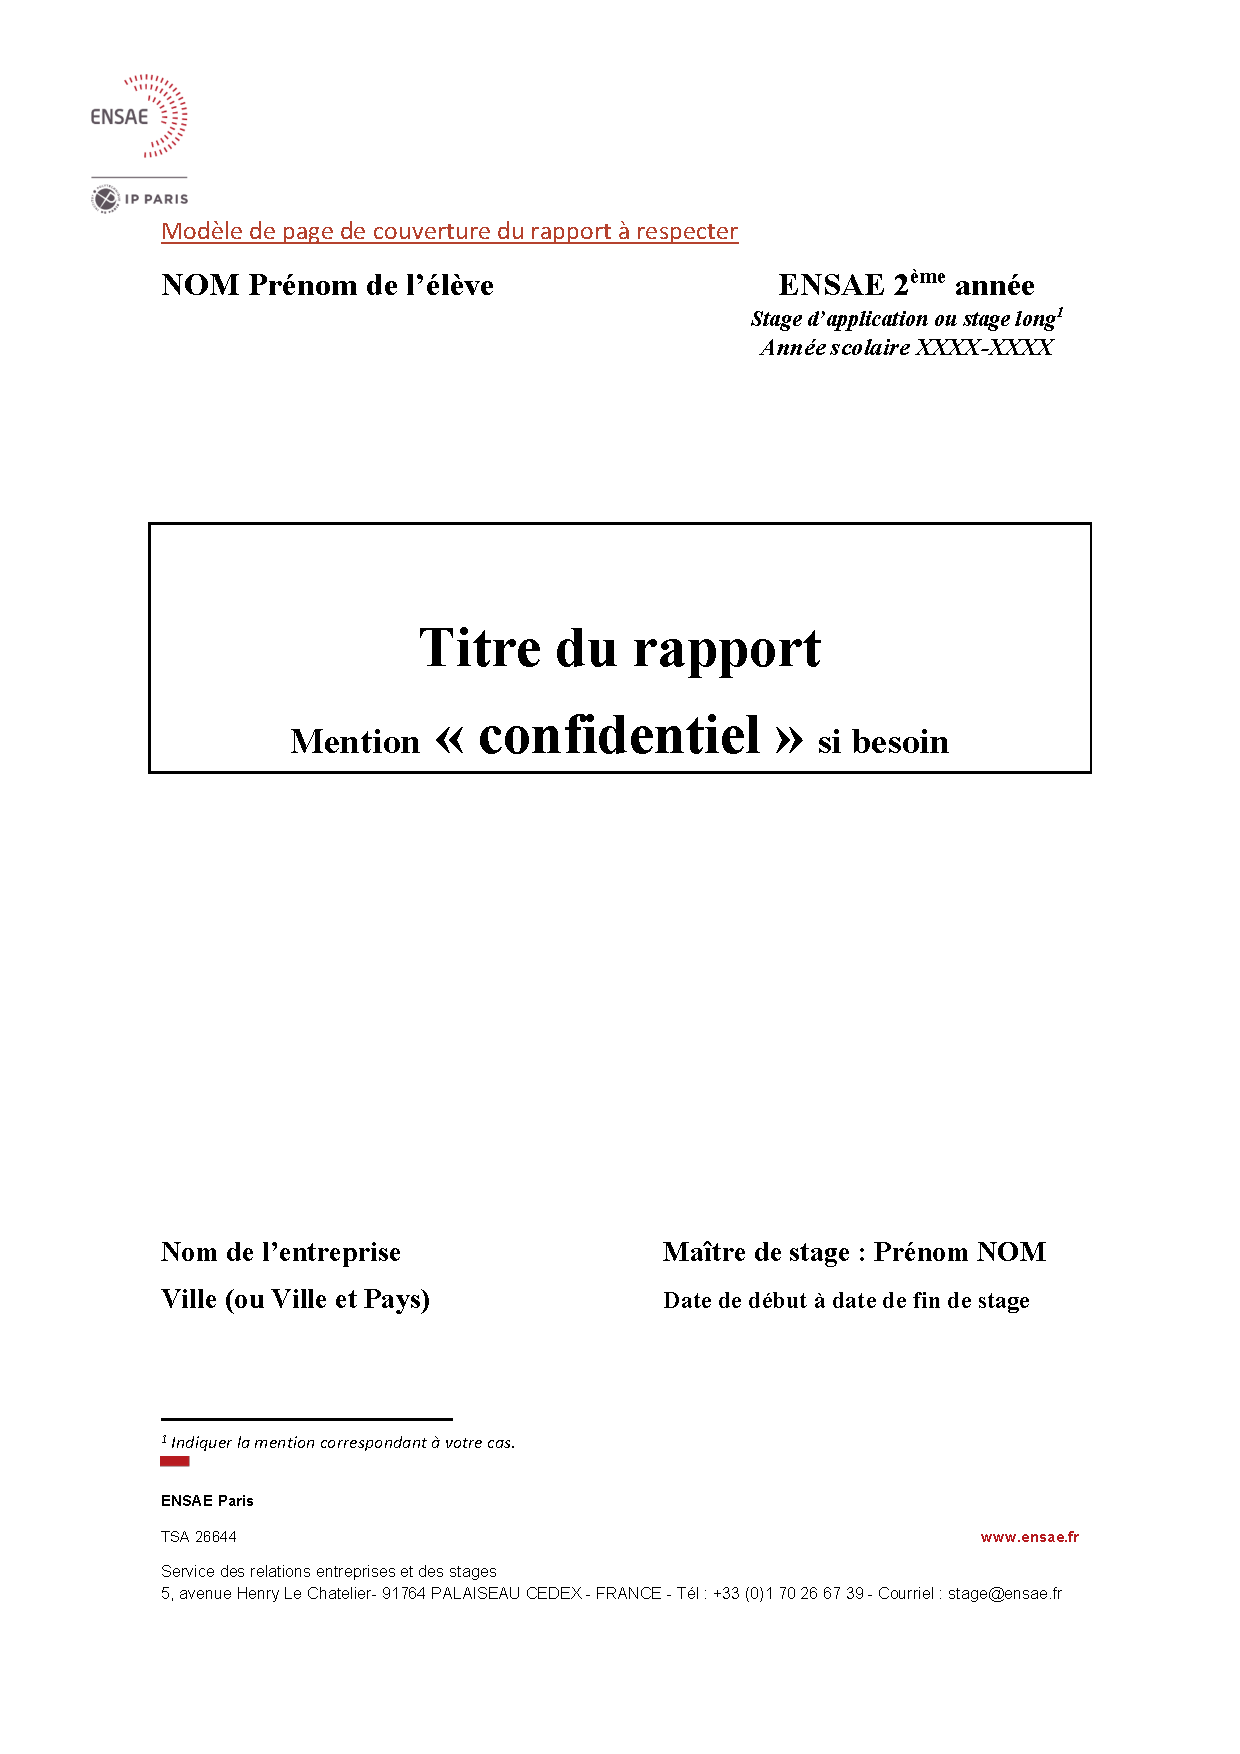
\includepdf[fitpaper=true, pages=-]{img/pdg.pdf}


\DeclareMathOperator{\e}{e}
\renewcommand{\P}{\mathds{P}} %Apparement \P existe déjà ?
\newcommand\N{\mathds{N}}
\newcommand\R{\mathds{R}}
%\newcommand\C{\mathds{C}}
%\newcommand\Z{\mathds{Z}}


\newcommand\1{\mathds{1}}
\newcommand{\E}[2][]{{\mathds{E}}_{#1}
  \def\temp{#2}\ifx\temp\empty
  \else
  \left[#2\right]
  \fi
}
\newcommand{\V}[2][]{{\mathds{V}}_{#1}
  \def\temp{#2}\ifx\temp\empty
  \else
  \left[#2\right]
  \fi
}
\newcommand\ud{\,\mathrm{d}}
\usepackage{booktabs}
\usepackage{longtable}
\usepackage{array}
\usepackage{multirow}
\usepackage{wrapfig}
\usepackage{float}
\usepackage{colortbl}
\usepackage{pdflscape}
\usepackage{tabu}
\usepackage{threeparttable}
\usepackage{threeparttablex}
\usepackage[normalem]{ulem}
\usepackage{makecell}
\usepackage{xcolor}
\ifxetex
  % Load polyglossia as late as possible: uses bidi with RTL langages (e.g. Hebrew, Arabic)
  \usepackage{polyglossia}
  \setmainlanguage[]{}
\else
  \usepackage[shorthands=off,main=]{babel}
\fi
\usepackage[style=authoryear,]{biblatex}
\addbibresource{biblio.bib}

\title{Rapport}
\author{Alain Quartier-la-Tente}
\date{6/17/2020}

\begin{document}
\maketitle

{
\hypersetup{linkcolor=}
\setcounter{tocdepth}{3}
\tableofcontents
}
\newpage

\hypertarget{introduction}{%
\section{Introduction}\label{introduction}}

\textcite{ch14HBSA}

\hypertarget{moving-average-and-filters}{%
\section{Moving average and filters}\label{moving-average-and-filters}}

A lot of papers describes the defi fnition and the properties of moving average and linear filters (see for example \textcite{ch12HBSA}).
Here we summarize some of the main results.

Let \(p\) et \(f\) two integers, a moving average \(M_\theta\) or \(M\) is defined by a set of coefficients \(\theta=(\theta_{-p},\dots,\theta_{f})'\) such as:
\[
M_\theta(X_t)=\sum_{k=-p}^{+f}\theta_kX_{t+k}
\]

\begin{itemize}
\item
  \(p+f+1\) is called the \emph{moving average order}.
\item
  When \(p=f\) the moving average is said to be \emph{centered}.
  If we also have \(\forall k:\:\theta_{-k} = \theta_k\), the moving average \(M_\theta\) is said to be \emph{symmetric}.
  In this case, the quantity \(h=p=f\) is called the \emph{bandwith}.
\end{itemize}

\hypertarget{gain-and-phase-shift-functions}{%
\subsection{Gain and phase shift functions}\label{gain-and-phase-shift-functions}}

Let \(X_t=\e^{i\omega t}\), the result of the moving average \(M_\theta\) in \(X_t\) is:
\[
Y_t = M_{\theta}X_t = \sum_{k=-p}^{+f} \theta_k \e^{i \omega (t+k)}
= \left(\sum_{k=-p}^{+f} \theta_k \e^{i \omega k}\right)\cdot X_t.
\]
The function \(\Gamma_\theta(\omega)=\sum_{k=-p}^{+f} \theta_k e^{i \omega k}\) is called the \emph{transfer function}.
It can be rewritten as:
\[
\Gamma_\theta(\omega) = G_\theta(\omega)\e^{-i\Phi_\theta(\omega)}
\]
where \(G_\theta(\omega)=\lvert\Gamma_\theta(\omega)\rvert\) is the \emph{gain} or \emph{amplitude} function and \(\Phi_\theta(\omega)\) is the \emph{phase shift} or \emph{time shift} function\footnote{This function is sometimes represented as \(\phi_\theta(\omega)=\frac{\Phi_\theta(\omega)}{\omega}\) to mesure the phase shift in number of periods.}.
For all symmetric moving average we have \(\Phi_\theta(\omega)=0\).

To sum up, applying a moving average to an harmonic times series affects in in two different ways:

\begin{itemize}
\item
  by multiplying it by an amplitude coefficient \(G_{\theta}\left(\omega\right)\);
\item
  by ``shifting'' it in time by \(\Phi_\theta(\omega)/\omega\), which directly affects the detection of turning points\footnote{When \(\Phi_\theta(\omega)/\omega>0\) the time shift is positive: a turning point is detected with delay.}.
\end{itemize}

Example: with \(M_{\theta_0}X_t=\frac{1}{2}X_{t-1}+\frac{1}{2}X_{t}\) we have:
\[
\Gamma_{\theta_0}(\omega)=\frac{1}{2}+\frac{1}{2}\e^{-i\omega}
=\lvert\cos(\omega/2)\rvert\e^{-i\frac{\omega}{2}}
\]
The figure \ref{fig:exgainPhase} illustrates the gain and the phase shift for \(\omega=\pi/2\) and \(X_t=\sin(\omega t)\).

\begin{figure}[!ht]
\pgfplotsset{width=\textwidth,height=6cm,every axis legend/.append style={font=\footnotesize,
  at={(0.5,-0.1)},
  anchor=north}
    }
\begin{tikzpicture}
\begin{axis}[
legend columns=2,
legend style = {fill=none , fill opacity=0, draw opacity=1,text opacity=1},
xtick={0,3.14159,...,15.70795},
xticklabels={0,$\pi$,$2\pi$,$3\pi$,$4\pi$,$5\pi$} 
]
\addplot[domain=0:5*pi,smooth,samples=300]    plot (\x,{sin(\x * (pi/2) r)});
\addlegendentry{$X_t(\pi/2)$}
\addplot[domain=0:5*pi,smooth,samples=300, dashed]    
  plot (\x,{1/2*sin(\x* pi/2 r )+1/2*sin((\x -1) * pi/2 r)});
\addlegendentry{$M_{\theta_0}X_t(\pi/2)$}
\draw[<->](axis cs: 1.5,1)--(axis cs: 1.5,0.7071068)
  node[pos=0.5, right]{\scriptsize $G_{\theta_0}(\pi/2)$};
\draw[<->] (axis cs: 3, -0.70710680-0.05)--(axis cs: 3.5,-0.7071068-0.05) 
  node[pos=0.5, below right]{\scriptsize $\Phi_{\theta_0}(\pi/2)$};
\end{axis}
\end{tikzpicture}
\caption{Smoothing of the time series $X_t=\sin(\omega t)$ by the moving average $M_{\theta_0}X_t=\frac{1}{2}X_{t-1}+\frac{1}{2}X_{t}$ for $\omega=\pi/2$.}\label{fig:exgainPhase}
\end{figure}

\hypertarget{desirable-properties-of-a-moving-average}{%
\subsection{Desirable properties of a moving average}\label{desirable-properties-of-a-moving-average}}

The moving average are often constructed under some specific constraints.
In the report we will focus on two constraints:

\begin{itemize}
\item
  the preservation of certain kind of trends;
\item
  the variance reduction.
\end{itemize}

\hypertarget{trend-preservation}{%
\subsubsection{Trend preservation}\label{trend-preservation}}

Is is often desirable for a moving average to conserve certain kind of trends.
A moving average \(M_\theta\) conserve a function of the time \(f(t)\) if \(\forall t:\:M_\theta f(t)=f(t)\).

We have the following properties for the moving average \(M_\theta\):

\begin{itemize}
\item
  To conserve a constant series \(X_t=a\) we need
  \[
  \forall t:M_\theta(X_t)=\sum_{k=-p}^{+f}\theta_kX_{t+k}=\sum_{k=-p}^{+f}\theta_ka=a\sum_{k=-p}^{+f}\theta_k=a
  \]
  the sum of the coefficients of the moving average \(\sum_{k=-p}^{+f}\theta_k\) must then be equal to \(1\).
\item
  To conserve a linear trend \(X_t=at+b\) we need:
  \[
  \forall t:\:M_\theta(X_t)=\sum_{k=-p}^{+f}\theta_kX_{t+k}=\sum_{k=-p}^{+f}\theta_k[a(t+k)+b]=at\sum_{k=-p}^{+f}k\theta_k+b\sum_{k=-p}^{+f}\theta_k=at+b
  \]
  which is equivalent to:
  \[
  \sum_{k=-p}^{+f}\theta_k=1
  \quad\text{and}\quad
  \sum_{k=-p}^{+f}k\theta_k=0
  \]
\item
  In general, it can be shown that \(M_\theta\) conserve a polynomial of degree \(d\) if and only if:
  \[
  \sum_{k=-p}^{+f}\theta_k=1 
   \text{ and } 
  \forall j \in \left\llbracket 1,d\right\rrbracket:\:
  \sum_{k=-p}^{+f}k^j\theta_k=0
  \]
\end{itemize}

\hypertarget{variance-reduction}{%
\subsubsection{Variance reduction}\label{variance-reduction}}

All time series are affected by noise that can blur the signal extraction.
Hence, we seek to reduce the variance of the noise.
The sum of the sum of the squares of the coefficients \(\sum_{k=-p}^{+f}\theta_k^2\) is the \emph{variance reduction} ratio.

Indeed, let \(\{\varepsilon_t\}\) a sequence of independent random variables with\(\E{\varepsilon_t}=0 \E{}\), \(\V{\varepsilon_t}=\sigma^2\).
\[
\V{M_\theta\varepsilon_t}=\V{\sum_{k=-p}^{+f} \theta_k \varepsilon_{t+k}}
= \sum_{k=-p}^{+f} \theta_k^2 \V{\varepsilon_{t+k}}=
\sigma^2\sum_{k=-p}^{+f} \theta_k^2
\]

\hypertarget{defAsymProb}{%
\subsection{Real-time estimation and asymmetric moving average}\label{defAsymProb}}

For symmetric filters, the phase shift function is equal to zero.
Therefore, there is no delay in any frequency: that's why they are prefered to the asymmetric one.
However, they cannot be used in the beginning and in the end of the time series because no past/future value can be used.
Thus, for real-time estimation, it is needed to build asymmetric moving average that approximate the symmetric moving average.

\textcite{ch15HBSA} \textcite{ch16HBSA,ch15HBSA}

\citeauthor*{ch15HBSA}

\citeyear{ch15HBSA}

\parencite{ch15HBSA}

\colorbox{BurntOrange}{à compléter}

\hypertarget{timeliness-guguemos}{%
\subsubsection{Timeliness (guguemos)}\label{timeliness-guguemos}}

timeliness
\[
\int_{\omega_{1}}^{\omega_{2}}f(\rho_{\theta}(\omega),\varphi_{\theta}(\omega))\ud\omega
\]

\hypertarget{quality-indicators-trouver-un-autre-nom}{%
\subsection{Quality indicators (? trouver un autre nom)}\label{quality-indicators-trouver-un-autre-nom}}

To compare the different moving average / filters the following indicators are used:

\begin{table}[!ht]
$$
\begin{array}{ccc}
\hline \text{Sigle} & \text{Description} & \text{Formula}\\
\hline b_{c} & \text{constant bias} & \sum_{k=-p}^{+f}\theta_{k}-1\\
\hline b_{l} & \text{linear bias} & \sum_{k=-p}^{+f}k\theta_{k}\\
\hline b_{q} & \text{quadratic bias} & \sum_{k=-p}^{+f}k^{2}\theta_{k}\\
\hline F_{g} & \text{variance reduction / fidelity} & \sum_{k=-p}^{+f}\theta_{k}^{2}\\
\hline S_{g} & \text{Smoothness} & \sum_{j}(\nabla^{3}\theta_{j})^{2}\\
\hline T_{g} & \text{Timeliness (Guguemos)} & \int_{0}^{\omega_{1}}\rho_{\theta}(\omega)\left|\varphi_{\theta}(\omega)\right|^{2}\ud\omega\\
\hline A_{w} & \text{Accuracy (Wildi)} & \int_0^{\omega_1}\left(A(\omega)-\hat{A}(\omega)\right)^{2}h(\omega)\ud\omega\\
\hline T_{w} & \text{Timeliness (Wildi)} & \int_0^{\omega_1} A(\lambda)\hat{A}(\lambda)\sin^{2}\left(\frac{\Phi(\omega)-\hat{\Phi}(\omega)}{2}\right)h(\omega)\ud\omega\\
\hline S_{w} & \text{Smoothness (Wildi)} & \int_{\omega_1}^{\pi}\left(A(\omega)-\hat{A}(\omega)\right)^{2}h(\omega)\ud\omega\\
\hline R_{w} & \text{Residual (Wildi)} & \int_{\omega_1}^{\pi} A(\lambda)\hat{A}(\lambda)\sin^{2}\left(\frac{\Phi(\omega)-\hat{\Phi}(\omega)}{2}\right)h(\omega)\ud\omega\\
\hline \\
\end{array}
$$
\caption{Quality criteria}
\footnotesize
\emph{Note: $X_g$ from \textcite{ch15HBSA} and $X_g$ from \textcite{trilemmaWMR2019}}
\end{table}

\colorbox{BurntOrange}{à compléter}

\hypertarget{local-polynomial-filters}{%
\section{Local polynomial filters}\label{local-polynomial-filters}}

In this section we detail the filters that arised from fitting a local polynomial to our time series, as described by \textcite{proietti2008}.

We assume that our time series \(y_t\) can be decomposed as
\[
y_t=\mu_t+\varepsilon_t
\]
where \(\mu_t\) is the signal (trend) and \(\varepsilon_{t}\overset{i.i.d}{\sim}\mathcal{N}(0,\sigma^{2})\) is the noise.
We assume that \(\mu_t\) can be locally approximated by a polynomial of degree \(d\) of the time \(t\) between \(y_t\) and the neighboring observations \(\left(y_{t+j}\right)_{j\in\left\llbracket -h,h\right\rrbracket}\). Then \(\mu_t\simeq m_{t}\) with:
\[
\forall j\in\left\llbracket -h,h\right\rrbracket :\:
y_{t+j}=m_{t+j}+\varepsilon_{t+j},\quad m_{t+j}=\sum_{i=0}^{d}\beta_{i}j^{i}
\]
This signal extraction problem is then equivalent to the estimation of \(m_t=\beta_0\). In matrix notation we can write:
\[
\underbrace{\begin{pmatrix}y_{t-h}\\
y_{t-(h-1)}\\
\vdots\\
y_{t}\\
\vdots\\
y_{t+(h-1)}\\
y_{t+h}
\end{pmatrix}}_{y}=\underbrace{\begin{pmatrix}1 & -h & h^{2} & \cdots & (-h)^{d}\\
1 & -(h-1) & (h-1)^{2} & \cdots & (-(h-1))^{d}\\
\vdots & \vdots & \vdots & \cdots & \vdots\\
1 & 0 & 0 & \cdots & 0\\
\vdots & \vdots & \vdots & \cdots & \vdots\\
1 & h-1 & (h-1)^{2} & \cdots & (h-1)^{d}\\
1 & h & h^{2} & \cdots & h^{d}
\end{pmatrix}}_{X}\underbrace{\begin{pmatrix}\beta_{0}\\
\beta_{1}\\
\vdots\\
\vdots\\
\vdots\\
\vdots\\
\beta_{d}
\end{pmatrix}}_{\beta}+\underbrace{\begin{pmatrix}\varepsilon_{t-h}\\
\varepsilon_{t-(h-1)}\\
\vdots\\
\varepsilon_{t}\\
\vdots\\
\varepsilon_{t+(h-1)}\\
\varepsilon_{t+h}
\end{pmatrix}}_{\varepsilon}
\]
Two parameters are crucial in determining the accuracy of the approximation:

\begin{itemize}
\item
  the degree \(d\) of the polynomial;
\item
  the number of neighbored \(H=2h+1\) (or the \emph{bandwith} \(h\)).
\end{itemize}

In order to estimate \(\beta\) we need \(H\geq d+1\) and the estimation is done by the weighted least squares (WLS), which consists of minimizing the following objective function:
\[
S(\hat{\beta}_{0},\dots,\hat{\beta}_{d})=\sum_{j=-h}^{h}\kappa_{j}(y_{t+j}-\hat{\beta}_{0}-\hat{\beta}_{1}j-\dots-\hat{\beta}_{d}j^{d})^{2}
\]
where \(\kappa_j\) is a set of weights called \emph{kernel}. We have \(\kappa_j\geq 0\), \(\kappa_{-j}=\kappa_j\) and with \(K=diag(\kappa_{-h},\dots,\kappa_{h})\), the estimate of \(\beta\) can be written as \(\hat{\beta}=(X'KX)^{1}X'Ky\).
With \(e_{1}=\begin{pmatrix}1&0&\cdots&0\end{pmatrix}'\), the estimate of the trend is:
\[
\hat{m}_{t}=e_{1}\hat{\beta}=w'y=\sum_{j=-h}^{h}w_{j}y_{t-j}\text{ with }w=KX(X'KX)^{-1}e_{1}
\]
To conclude, the estimate of the trend \(\hat{m}_{t}\) can be obtained applying the symmetric filter \(w\) to \(y_t\)\footnote{\(w\) is symmetric due to the symmetry of the kernel weights \(\kappa_j\).}.
Moreover, \(X'w=e_{1}\) so:
\[
\sum_{j=-h}^{h}w_{j}=1,\quad\forall r\in\left\llbracket 1,d\right\rrbracket :\sum_{j=-h}^{h}j^{r}w_{j}=0
\]
Hence, the filter \(w\) preserve deterministic polynomial of order \(d\).

\hypertarget{sec:kernels}{%
\subsection{Different kernels}\label{sec:kernels}}

In signal extraction, we generally look for weighting observations according to their distance from time \(t\): this is the role of the kernel function.
For that, we introduce a kernel function \(\kappa_j\), \(j=0,\pm1,\dots,\pm h\) with \(\kappa_j \geq0\) and \(\kappa_j=\kappa_{-j}\).
An important class of kernels is the Beta kernels. In the discrete, up to a proportional factor (so that \(\sum_{j=-h}^h\kappa_j=1\)):
\[
\kappa_j = \left(
  1-
  \left\lvert
  \frac j {h+1}
  \right\lvert^r
\right)^s
\]
with \(r>0\), \(s\geq 0\). The following kernels are considered in this report:

\begin{multicols}{2}
\begin{itemize}
\item $r=1,s=0$ uniform kernel: 
$$\kappa_j^U=1$$
\item $r=s=1$ triangle kernel:
$$\kappa_j^T=\left(
  1-
  \left\lvert
  \frac j {h+1}
  \right\lvert
\right)$$

\item $r=2,s=1$  Epanechnikov (or Parabolic) kernel:
$$\kappa_j^E=\left(
  1-
  \left\lvert
  \frac j {h+1}
  \right\lvert^2
\right)$$

\item $r=s=2$ biweight kernel:
$$\kappa_j^{BW}=\left(
  1-
  \left\lvert
  \frac j {h+1}
  \right\lvert^2
\right)^2$$

\item $r = 2, s = 3$ triweight kernel:
$$\kappa_j^{TW}=\left(
  1-
  \left\lvert
  \frac j {h+1}
  \right\lvert^2
\right)^3$$

\item $r = s = 3$ tricube kernel:
$$\kappa_j^{TC}=\left(
  1-
  \left\lvert
  \frac j {h+1}
  \right\lvert^3
\right)^3$$

\item Gaussian kernel\footnote{
The gaussian kernel is generally defined as $\e^{-\frac{ x^2}{ 2\sigma^2}}$.
Here we take $\sigma^2=2/h$ with the following idea: the biggest $h$ is, the narrowest the filter is.
}:
$$
\kappa_j^G=\exp\left(
-\frac{
  j^2
}{
  4h
}\right)
$$
\item Henderson kernel (see section \ref{sec:sympolyfilter} for its construction):
$$
\kappa_{j}=\left[1-\frac{j^2}{(h+1)^2}\right]
\left[1-\frac{j^2}{(h+2)^2}\right]
\left[1-\frac{j^2}{(h+3)^2}\right]
$$
\item Trapezoidal kernel:
$$
\kappa_j^{TP}=
\begin{cases}
  \frac{1}{3(2h-1)} & \text{ if }j=\pm h 
  \\
  \frac{2}{3(2h-1)} & \text{ if }j=\pm (h-1)\\
  \frac{1}{2h-1}& \text{ otherwise}
\end{cases}
$$
\end{itemize}
\end{multicols}

The figure \ref{fig:kernels} summarises the coefficients of the different kernels.
Analysing the coefficients we can already anticipate some properties of the associated filters:

\begin{itemize}
\item
  For \(h\) small the triweight kernel has the narrowest distribution, for \(h\) high (\(h\geq15\)) the gaussian kernel become narrowest.
  The narrowest a distribution is, the smallest the weights of furthest neighbors are: the associated filter should have a high weight in the current observation (\(t\)).
\item
  For \(h\) high the Henderson kernel is equivalent to the triweight kernel (since \(h+1\sim h+2 \sim h+3\), \(\kappa_j^H\sim\kappa_j^{TW}\)), the associated filter should also be equivalent.
\end{itemize}

\begin{figure}[!ht]
\animategraphics[autoplay,loop,width=\textwidth,controls]{2}{img/kernels/}{2}{30} 
\caption{Coefficients of the different kernels for $h$ from 2 to 30.}\label{fig:kernels}\footnotesize
\emph{Note: to see the animation the PDF must be open with Acrobat Reader, KDE Okular, PDF-XChange or Foxit Reader. 
Otherwise you will only be able to see the results for $h=2$.}
\end{figure}

\hypertarget{sec:sympolyfilter}{%
\subsubsection{Specific symmetric filters}\label{sec:sympolyfilter}}

When \(p=0\) (local adjustment by a constant) we obtain the \textbf{Nadaraya-Watson}'s estimator.

With the uniform kernel we obtain the \textbf{Macaulay filter}. When \(p=0,1\), this is the arithmetic moving average: \(w_j=w=\frac{1}{2h+1}\).

The \textbf{Epanechnikov} kernel is often recommended as the optimal kernel that minimize the mean square error of the estimation by local polynomial.

\textbf{Loess} is a locally weighted polynomial regression that use tricube kernel.

The \textbf{Henderson filter} is a specific case of a local cubif fit (\(p=3\)).
It is often used Henderson for trend estimation (for example it's the filter used in the seasonal adjustment). For a fixed bandwith, Henderson found the kernel that gave the smoothest estimates of the trend.
He showed that the three following problems were equivalent:

\begin{enumerate}
\def\labelenumi{\arabic{enumi}.}
\tightlist
\item
  minimize the variance of third difference of the series by the application of the moving average;\\
\item
  minimize the sum of squares of third difference of the coefficients of the filter, it's the \emph{smothness criteria}: \(S=\sum_j(\nabla^{3}\theta_{j})^{2}\);\\
\item
  fit a local cubic polynomial by weighted least squares, where the weights are chose to minimize the sum of squares of the resulting filter.
\end{enumerate}

Resolving the last problem leads to the kernel presented in section \ref{sec:kernels}.

\hypertarget{analysis-of-symmetric-filters}{%
\subsubsection{Analysis of symmetric filters}\label{analysis-of-symmetric-filters}}

In this section, all the filters are computed by local polynomial of degree \(d=3\).
The figure~\ref{fig:filterscoefs} plots the coefficients of the filters for the differents kernels presented in different kernels presented in section \ref{sec:kernels} and for different bandwith \(h\).
The table \ref{tab:varianceReductionSymmetricFilters} shows the variance reduction of the different filters.
We find the similar results than in section~\ref{fig:kernels}:

\begin{itemize}
\item
  For \(h\) small the triweight kernel gives the filter with the narrowest distribution, for \(h\) high (\(h\geq15\)) the gaussian kernel become narrowest.
  The narrowest a distribution is, the higher the variance reduction should be.
  Indeed, the distribution of the coefficients of the filter can be interprated as the output signal of an additive outlier.
  As a result, with a wide distribution, an additive outlier will be more persistent than with a narrow distribution.
  Therefore, it's the triweight that has the higher variance reduction for all \(h\leq30\).
\item
  For \(h\) small, the trapezoidal filter seems to produce similar results than the Epanechnikov one.
\item
  For \(h\) high the Henderson filter is equivalent to the one computed by the triweight kernel.
\end{itemize}

\begin{figure}[!ht]
\animategraphics[autoplay,loop,width=\textwidth,controls]{2}{img/symmetricFilters/}{2}{30}
\caption{Coefficients of symmetric filters computed by local polynomial of degree $3$, according to the differents kernels and for $h$ from 2 to 30.}\label{fig:filterscoefs}\footnotesize
\emph{Note: to see the animation the PDF must be open with Acrobat Reader, KDE Okular, PDF-XChange or Foxit Reader.
Otherwise you will only be able to see the results for $h=2$.}
\end{figure}

Moreover, we find that for all the filters, the coefficients decrease, when the distance to the central observation increases, until a negative value and then increase towards 0 (except for the uniform kernel).
Negative coefficients might be disturbing but they arise from the cubic polynomial constraints.
Indeed to preserve polynomial of degree 2 (and so 3) we need \(\sum_{j=-h}^hj^2\theta_i=0\), which constraint some coefficients to be negative.
However, those negative coefficients are negligible compare to the central higher coefficients (they are more 80\% smaller than the central coefficient for all kernels, except for uniform and trapezoidal with high bandwith).

\begin{table}[!h]

\caption{\label{tab:varianceReductionSymmetricFilters}Variance reduction ratio ($\sum\theta_i^2$) of symmetric filters computed by local polynomial of degree $3$.}
\centering
\resizebox{\linewidth}{!}{
\begin{tabular}[t]{cccccccccc}
\toprule
\multicolumn{1}{c}{ } & \multicolumn{9}{c}{Kernel} \\
\cmidrule(l{3pt}r{3pt}){2-10}
$h$ & Biweight & Epanechnikov & Gaussian & Henderson & Trapezoidal & Triangular & Tricube & Triweight & Uniform\\
\midrule
\rowcolor{gray!6}  2 & 0.50 & 0.49 & 0.49 & 0.50 & 0.51 & 0.51 & 0.49 & 0.52 & 0.49\\
3 & 0.33 & 0.30 & 0.30 & 0.32 & 0.31 & 0.33 & 0.32 & 0.37 & 0.28\\
\rowcolor{gray!6}  4 & 0.25 & 0.23 & 0.24 & 0.25 & 0.23 & 0.25 & 0.25 & 0.28 & 0.22\\
5 & 0.22 & 0.21 & 0.21 & 0.22 & 0.20 & 0.22 & 0.22 & 0.24 & 0.20\\
\rowcolor{gray!6}  6 & 0.20 & 0.19 & 0.19 & 0.20 & 0.19 & 0.20 & 0.20 & 0.21 & 0.19\\
\addlinespace
7 & 0.19 & 0.18 & 0.18 & 0.19 & 0.18 & 0.19 & 0.19 & 0.20 & 0.18\\
\rowcolor{gray!6}  8 & 0.18 & 0.17 & 0.18 & 0.18 & 0.17 & 0.18 & 0.18 & 0.19 & 0.17\\
9 & 0.17 & 0.17 & 0.17 & 0.17 & 0.17 & 0.17 & 0.17 & 0.18 & 0.17\\
\rowcolor{gray!6}  10 & 0.17 & 0.16 & 0.17 & 0.17 & 0.16 & 0.17 & 0.17 & 0.17 & 0.16\\
20 & 0.12 & 0.12 & 0.13 & 0.13 & 0.12 & 0.12 & 0.13 & 0.13 & 0.12\\
\addlinespace
\rowcolor{gray!6}  30 & 0.10 & 0.10 & 0.10 & 0.10 & 0.10 & 0.10 & 0.10 & 0.10 & 0.10\\
\bottomrule
\end{tabular}}
\end{table}

\hypertarget{gain-functions}{%
\subsubsection{Gain functions}\label{gain-functions}}

Figure \ref{fig:filtersSymgains} plots the gain functions of the different filters.
Gain functions are usually plotted between 0 and \(\pi\).
However, locally weighted polynomial regression are low-pass filters: they leave almost unchanged low frequency components (such as the trend) and attenuate high frequency fluctuations (noise).
That's why we are only interested in low frequencies.
For a monthly data, a cycle of 3 years correspond to the frequency \(2\pi/36\) and a cycle of 7 years to the frequency \(2\pi/84\).

When the bandwith \(h\) increases, the gain function decreases for low frequencies: short business cycles will then be attenuated.
For a fixed value of \(h\), gaussian, Henderson and triweight filters will preserve more short business cycles than the others filters (especially uniform, trapezoidal and Epanechnikov).

\colorbox{BurntOrange}{tracer et interpréter gain après $2\pi/12$ pour voir à partir de quelles fréquences sont atténuées ?}
\colorbox{BurntOrange}{ou bien c'est résumé avec le pouvoir de réduction de la variance ?}

\begin{figure}[!ht]
\animategraphics[autoplay,loop,width=\textwidth,controls]{2}{img/symmetricFilters/gain}{2}{30}
\caption{Gain functions from 0 to $2\pi/12$ of symmetric filters computed by local polynomial of degree $3$, according to the differents kernels and for $h$ from 2 to 30.}\label{fig:filtersSymgains}\footnotesize
\emph{Note: to see the animation the PDF must be open with Acrobat Reader, KDE Okular, PDF-XChange or Foxit Reader.
Otherwise you will only be able to see the results for $h=2$.}
\end{figure}

\hypertarget{asymmetric-filters}{%
\subsection{Asymmetric filters}\label{asymmetric-filters}}

\hypertarget{direct-asymmetric-filters-daf}{%
\subsubsection{Direct asymmetric filters (DAF)}\label{direct-asymmetric-filters-daf}}

As mentionned in section \ref{defAsymProb}, symmetric filters cannot be used in boundary points. For real-time estimation, three different approaches can be used:

\begin{enumerate}
\def\labelenumi{\arabic{enumi}.}
\item
  Build a asymmetric filter fitting local polynomial to the available observations \(y_{t}\) for \(t\in\left\llbracket n-h,n\right\rrbracket\).
\item
  Apply the symmetric filter to the series extended by forecast (or backcast) \(\hat{y}_{n+l\mid n},l\in\left\llbracket 1,h\right\rrbracket\).
\item
  Build a asymmetric filter which minimize the mean square revision error subject to polynomial reproducing constraints.
\end{enumerate}

\textcite{proietti2008} show that the first two approaches are equivalent when the forecast is done by a polynomial extrapolation of order \(d\) (forecasts generated with the same polynomial model than the symmetric filter). This is called the \emph{direct asymmetric filter} (DAF).
Let \(q\) be the number of available observations in the future: \(q\) varies from 0 (real time filter) to \(h\) (symmetric filter).

Rewritting the matrix \(X\), \(K\) \(y\) in the following way:
\[
X=\begin{pmatrix}X_{p}\\
X_{f}
\end{pmatrix},\quad y=\begin{pmatrix}y_{p}\\
y_{f}
\end{pmatrix},\quad K=\begin{pmatrix}K_{p} & 0\\
0 & K_{f}
\end{pmatrix}
\]
where \(y_{p}\) correspond to the available data and \(y_{f}\) the missing data, the DAF \(w_a\) and the forecast \(\hat{y}_{f}\) can be written as:
\[
w_{a}=K_{p}X_{p}(X'_{p}K_{p}X_{p})^{-1}e_{1},
\quad
\hat{y}_{f}=X_{f}(X'_{p}K_{p}X_{p})^{-1}X_{p}'K_{p}y_{p}
\]
Moreover, we have the folliwing results with the DAF \(w_a\):

\begin{itemize}
\item
  it satisfy the same polynomial reproduction constraints as the symmetric filter (conserve polynomial of degree \(d\)).
  Thus, the bias in estimating an unknown function of time has the same order of magnitude as in the interior of time support.
\item
  \(w_a\) minimize the weighted distance (by the kernel function) between the asymmetric filter coefficients and the symmetric ones.
\end{itemize}

However, the weights \(w_{a,0}\) of the DAF are highly concentrated in the current observation \(t\) with an important change between \(q=0\) (real-time filter) and \(q=h\) (see figure \ref{filtersdafcoefs}).
Moroever the real-time filter doesn't have a satisfying gain functions: it is close to one for all the frequencies.
Therefore, even if the real-time filter is unbiased (if the series is generated by a polynomial of degree \(d\)) it is at the expenses of a high variance.

\begin{figure}[!ht]
\animategraphics[autoplay,loop,width=\textwidth,controls]{2}{img/daf/coef_gain_}{1}{9}
\caption{Coefficients and gain function of direct asymmetric filters (DAF) computed by local polynomial of degree $3$, according to the differents kernels and for $h=6$.}\label{fig:filtersdafcoefs}\footnotesize
\emph{Note: to see the animation the PDF must be open with Acrobat Reader, KDE Okular, PDF-XChange or Foxit Reader.
Otherwise you will only be able to see the results for the Henderson kernel.}
\end{figure}

For all the kernels, we find the same results as in \textcite{proietti2008}:

\begin{itemize}
\item
  For a fixed value of \(d\), the more the data is available (\(q\) increases), the more the weight associated to the current observation \(w_{a,0}\) decreases.
\item
  For a fixed value of \(h\) and \(q\), \(w_{a,0}\) increases exponentially with the polynomial degree \(d\) (in particular, for \(d=h\), \(w_{a,0}=1\)).
\end{itemize}

\hypertarget{general-class-of-asymmetric-filters}{%
\subsubsection{General class of asymmetric filters}\label{general-class-of-asymmetric-filters}}

To deal with the problem of the variance of the estimates of the real-time filters, \textcite{proietti2008} suggest a general of asymmetric filters to make a tradeoff between bias and variance.

Here we consider that the data is generated by the model:
\[
y=U\gamma+Z\delta+\varepsilon,\quad
\varepsilon\sim\mathcal{N}(0,D)
\]
The goal is to find a filter \(v\) which minimize the mean square revision error (with the symmetric filter \(w\)) subject to some constraints.
The constraints are summarized by the matrix \(U=\begin{pmatrix}U_{p}'&U_{f}'\end{pmatrix}'\) (with \(U_p\) the available observations of the matrix \(U\) for the asymmetric filter): \(U_p'v=U'w\).
The problem is equivalent to find \(v\) that minimize:
\[
\varphi(v)=
\underbrace{
  \underbrace{(v-w_{p})'D_{p}(v-w_{p})+
  w_{f}'D_{f}w_{f}}_\text{revision error variance}+
  \underbrace{[\delta'(Z_{p}'v-Z'w)]^{2}}_{biais^2}
}_\text{Mean square revision error}+
\underbrace{2l'(U_{p}'v-U'w)}_{\text{constraints}}
\]
with \(l\) a vector of Lagrange multipliers.

When \(U=X\) this is equivalent to the constraint to preserve polynomial of degree \(d\): we find the direct asymmetric filters \(w_a\) with \(D=K^{-1}\).

When \(U=\begin{pmatrix}1&\cdots&1\end{pmatrix}'\), \(Z=\begin{pmatrix}-h&\cdots&+h\end{pmatrix}'\), \(\delta=\delta_1\), \(D=\sigma^2I\) and when the symmetric filter is the Henderson filter we obtain the Musgrave asymmetric filters (see \colorbox{BurntOrange}{ajouter biblio}).
With the filter we assume that the data is generated by a linear process and that the asymmetric filters preserve constant signals (\(\sum v_i=\sum w_i=1\)).
The asymmetric filters depends on the ratio \(\delta_1/\sigma\), which is related to the ``I-C'' ratio \(R=\frac{\bar{I}}{\bar{C}}=\frac{\sum\lvert I_t-I_{t-1}\rvert}{\sum\lvert C_t-C_{t-1}\rvert}\) (\(\delta_1/\sigma=2/(R\sqrt{\pi})\)), the ratio between the expected absolute difference of the irregular and of the trend-cycle.
In the seasonal adjustment method, the I-C ratio\footnote{In order to compute the I-C ratio, a first decomposition of the seasonally adjusted series is computed using a 13-term Henderson moving average.} is used to determine the bandwith to used for the Henderson filter. For monthly data:

\begin{itemize}
\item
  if \(R<1\) a 9-term Henderson is used (\(h=4\));
\item
  if \(1\leq R\leq3.5\) a 13-term Henderson is used (\(h=6\));
\item
  if \(3.5< R\) a 23-term Henderson is used (\(h=12\)).
\end{itemize}

When \(U\) corresponds to the first \(d^*+1\) first the columns of \(X\), \(d^*<d\), the constraint is that the asymmetric filter should reproduce polynomial of degree \(d^*\), the potential bias depends on the value of \(\delta\).
This will reduce the variance at the expense of a bias: it is the idea followed by \textcite{proietti2008} to propose three class of asymmetric filters:

\begin{enumerate}
\def\labelenumi{\arabic{enumi}.}
\item
  \emph{Linear-Constant} (LC): \(y_t\) linear (\(d=1\)) and \(v\) preserve constant signals (\(d^*=0\)), \(v\) depend on the ratio \(\delta_1^2/\sigma^2\).
\item
  \emph{Quadratic-Linear} (QL): \(y_t\) quadratic (\(d=2\)) and \(v\) preserve linear signals (\(d^*=1\)), \(v\) depend on the ratio \(\delta_2^2/\sigma^2\).
\item
  \emph{Cubic-Quadratic} (CQ): \(y_t\) cubic (\(d=3\)) and \(v\) preserve linear signals (\(d^*=1\)), \(v\) depend on the ratio \(\delta_2^2/\sigma^2\).
\end{enumerate}

\begin{table}[!h]

\caption{\label{tab:criteriaLp}Quality criteria of real-time filters ($q=0$) computed by local polynomial.}
\centering
\resizebox{\linewidth}{!}{
\begin{tabular}[t]{cccccccccc}
\toprule
\multicolumn{1}{c}{ } & \multicolumn{9}{c}{Kernel} \\
\cmidrule(l{3pt}r{3pt}){2-10}
Criteria & Henderson & Gaussian & Trapezoidal & Triweight & Tricube & Biweight & Epanechnikov & Triangular & Uniform\\
\midrule
\addlinespace[0.3em]
\multicolumn{10}{l}{\textbf{LC}}\\
\hspace{1em}$ b_l $ & -0.407 & -0.415 & -0.450 & -0.387 & -0.414 & -0.411 & -0.438 & -0.409 & -0.467\\
\hspace{1em}$ b_q $ & -2.161 & -2.258 & -2.597 & -1.971 & -2.211 & -2.196 & -2.472 & -2.237 & -2.787\\
\hspace{1em}$ F_g $ & 0.388 & 0.384 & 0.377 & 0.396 & 0.387 & 0.387 & 0.379 & 0.385 & 0.376\\
\hspace{1em}$ S_g $ & 1.272 & 1.281 & 1.172 & 1.346 & 1.191 & 1.249 & 1.209 & 1.424 & 1.307\\
\hspace{1em}$ T_g \times 10^{-3} $ & 30.341 & 32.469 & 40.848 & 26.230 & 31.654 & 31.174 & 37.673 & 31.686 & 45.669\\
\addlinespace[0.3em]
\multicolumn{10}{l}{\textbf{QL}}\\
\hspace{1em}$ b_q $ & -0.473 & -0.488 & -0.545 & -0.441 & -0.483 & -0.479 & -0.524 & -0.482 & -0.574\\
\hspace{1em}$ F_g $ & 0.711 & 0.708 & 0.702 & 0.716 & 0.712 & 0.711 & 0.704 & 0.708 & 0.697\\
\hspace{1em}$ S_g $ & 5.149 & 5.207 & 5.499 & 5.011 & 5.172 & 5.181 & 5.369 & 5.436 & 5.546\\
\hspace{1em}$ T_g \times 10^{-3} $ & 0.047 & 0.054 & 0.089 & 0.036 & 0.052 & 0.050 & 0.074 & 0.055 & 0.111\\
\addlinespace[0.3em]
\multicolumn{10}{l}{\textbf{CQ}}\\
\hspace{1em}$ F_g $ & 0.913 & 0.913 & 0.914 & 0.913 & 0.912 & 0.913 & 0.913 & 0.914 & 0.915\\
\hspace{1em}$ S_g $ & 11.942 & 11.918 & 12.201 & 11.803 & 12.122 & 11.995 & 12.097 & 12.039 & 12.062\\
\hspace{1em}$ T_g \times 10^{-3} $ & 0.015 & 0.015 & 0.012 & 0.016 & 0.014 & 0.014 & 0.013 & 0.014 & 0.013\\
\addlinespace[0.3em]
\multicolumn{10}{l}{\textbf{DAF}}\\
\hspace{1em}$ F_g $ & 0.943 & 0.939 & 0.930 & 0.952 & 0.942 & 0.942 & 0.933 & 0.940 & 0.929\\
\hspace{1em}$ S_g $ & 14.203 & 13.968 & 12.699 & 15.002 & 13.881 & 14.040 & 13.140 & 14.298 & 12.422\\
\hspace{1em}$ T_g \times 10^{-3} $ & 0.003 & 0.004 & 0.008 & 0.001 & 0.003 & 0.003 & 0.006 & 0.004 & 0.012\\
\bottomrule
\end{tabular}}
\end{table}

\ref{fig:filtersasymErr}:

\begin{itemize}
\item
  almost same symmetric trend for all the filters: small differences during ``turning points''.
  Differences less than one point for between all the kernels, uniform and trapezoidal more ``atypical'', Differences less than 0,5 point for the other kernels.
  Différences p/r Henderson toujours dans le même sens sauf pour triweight (?) : sous Henderson pendant les ``cycles bas'', au-dessus pendant ``cycles hauts''
\item
  revisions error are higher with uniform and trapezoidal kernels, lower with triweight, regardless of the asymmetric filter.
\item
  in mean, the variance revision error is always lower with the LC filter and higher with the DAF. However, during turning-points (for example around the 2008 crisis), the LC filter have a higher bias than the other filters. For the French IPI, the CQ method seems to give the better results around the 2008 crisis (analyzing mean squared error revision between 2007 and 2011). However, reproducing the same procedure to the IPI of other countries of the European Union (and the United-Kingdom), we find that for most of the series (23 of 28) its the QL filter that gives the better results during the 2008 crisis.
\end{itemize}

\begin{figure}[!ht]
\animategraphics[autoplay,loop,width=\textwidth,controls]{2}{img/daf/comp_assym_}{1}{9}
\caption{Revision error of the different real-time ($q=0$) asymmetric filters for $h=6$, for the IPI-FR.}\label{fig:filtersasymErr}\footnotesize
\emph{Note: to see the animation the PDF must be open with Acrobat Reader, KDE Okular, PDF-XChange or Foxit Reader.
Otherwise you will only be able to see the results for the Henderson kernel.}
\end{figure}

\newpage

\printbibliography[title=References]

\end{document}
